\documentclass{standalone}
\usepackage{tikz}
\usetikzlibrary{positioning}
\begin{document}
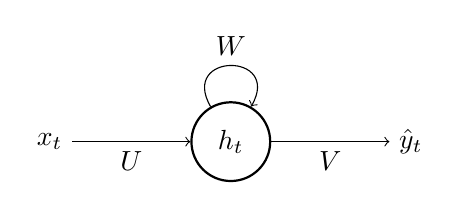
\begin{tikzpicture}[
    node distance = 1.5cm,
    roundnode/.style={circle, draw=black, fill=white, thick, minimum size=10mm},
  ]
  % RNN iamge
  \node (xt) {$x_t$};
  \node[roundnode] (ht) [right=of xt] {$h_t$};
  \node (yt) [right=of ht] {$\hat{y}_t$};

  \draw[->] (xt) -- node[below] {$U$} (ht);
  \draw[->] (ht) -- node[below] {$V$} (yt);
  \draw[->] (ht) to [out=120, in=60, looseness=4] node [above] {$W$} (ht);
\end{tikzpicture}
\end{document}


